\section{全データへの適用}
\label{sec_full}
\subsection{処理の実績}
最終の構成を BoketeDBv4 の全てのお題画像に適用した．
予測の段階では，6,609,511枚の代表画像を36,634秒，すなわち約10.2時間で処理し，速度は毎秒約180枚であった．
無作為の2万枚での測定より速いのは，画像の読み込みのプロセス数を増やしたためである．
確認の質問の対象は，形式がお題文と予測された551,260枚であり，代表画像の8.3\%であった．
本稿の執筆の時点で，確認の段階は対象のうち320,000枚を処理しており，速度は毎秒約33枚であった．
この速度では，確認の段階の全体に約4.7時間を要する．
したがって，以下に示す全データの集計は，確認の質問を適用する前の予測による．
確認の質問で形式が変わる画像は，無作為の2万枚で約0.05\%であったため，以下の集計への影響は小さいと見込まれる．

\subsection{ラベルの分布}
表\ref{tab_full_dist}に，全6,823,270件のお題におけるラベルの割合を示す．
比較のため，実データの無作為抽出160枚の目視ラベルの割合も示す．

\begin{table}[t]
    \centering
    \caption{全データにおけるラベルの割合（確認の質問の前の予測）}
    \label{tab_full_dist}
    \small
    \begin{tabular}{llcc}
        \toprule
        軸 & 項目 & 全データ & 目視（160枚） \\
        \midrule
        \multirow{4}{*}{形式} & カルタ & 1.1\% & 1.9\% \\
         & 穴埋め & 20.1\% & 19.4\% \\
         & お題文 & 8.3\% & 6.9\% \\
         & 通常 & 70.5\% & 71.9\% \\
        \midrule
        \multirow{3}{*}{属性} & 空欄あり & 21.4\% & -- \\
         & カルタ記号あり & 1.1\% & -- \\
         & 文字あり & 58.6\% & 60.6\% \\
        \midrule
        \multirow{7}{*}{媒体} & 写真 & 53.1\% & 53.7\% \\
         & アニメ & 9.1\% & 8.1\% \\
         & ゲーム & 2.3\% & 2.5\% \\
         & マンガ & 15.2\% & 16.3\% \\
         & テキストグラフィック & 14.5\% & 14.4\% \\
         & 絵画 & 0.9\% & 0.0\% \\
         & イラスト & 11.2\% & 10.6\% \\
        \midrule
        \multicolumn{2}{l}{媒体を2つ以上選んだ画像} & 6.0\% & 6.3\% \\
        \bottomrule
    \end{tabular}
\end{table}

全データの分布は，160枚の目視ラベルの分布とおおむね一致した．
お題の約3割は通常以外の形式であり，そのうち穴埋めが約2割と最も多い．
お題文は目視ラベルよりやや高く，これは確認の質問の前の予測であることと，\ref{sec_final}章で示したお題文の適合率の限界による．
媒体では，写真が約半数を占め，作品の知識を前提としうるアニメ，マンガ，ゲーム，絵画の割合の合計は，複数選択を重複して数えて約28\%であった．
文字ありは約59\%であり，画像の過半数に何らかの読める文字が含まれる．

\subsection{投稿年ごとの推移}
図\ref{fig_full_year_format}に，投稿年ごとの通常以外の形式の割合を示す．
横軸はお題の投稿年，縦軸はその年に投稿されたお題に占める割合である．
2026年はデータの収集の時点までの値である．

\begin{figure}[t]
    \centering
    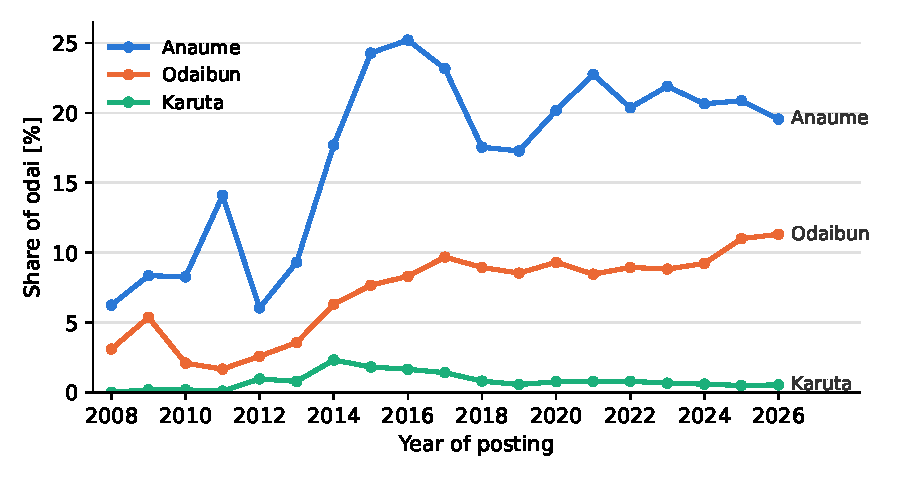
\includegraphics[width=\linewidth]{figures/fig_full_year_format.pdf}
    \caption{投稿年ごとの形式の割合．Anaume は穴埋め，Odaibun はお題文，Karuta はカルタを表す}
    \label{fig_full_year_format}
\end{figure}

穴埋めの割合は2013年以前は6\%から14\%であったが，2014年から急増し，2016年に25.2\%で最大となった．
その後は17\%から23\%で推移している．
お題文の割合は2013年以前は2\%から5\%であったが，その後は徐々に増え，2025年以降は約11\%となった．
カルタは2014年の2.3\%が最大であり，近年は1\%未満である．
2008年から2012年は年間のお題数が2万件から10万件程度と少なく，割合の変動が大きい．

図\ref{fig_full_year_media}に，投稿年ごとの媒体と文字ありの割合を示す．
各図の横軸は投稿年，縦軸はその年のお題に占める割合であり，縦軸の範囲は図ごとに異なる．

\begin{figure*}[t]
    \centering
    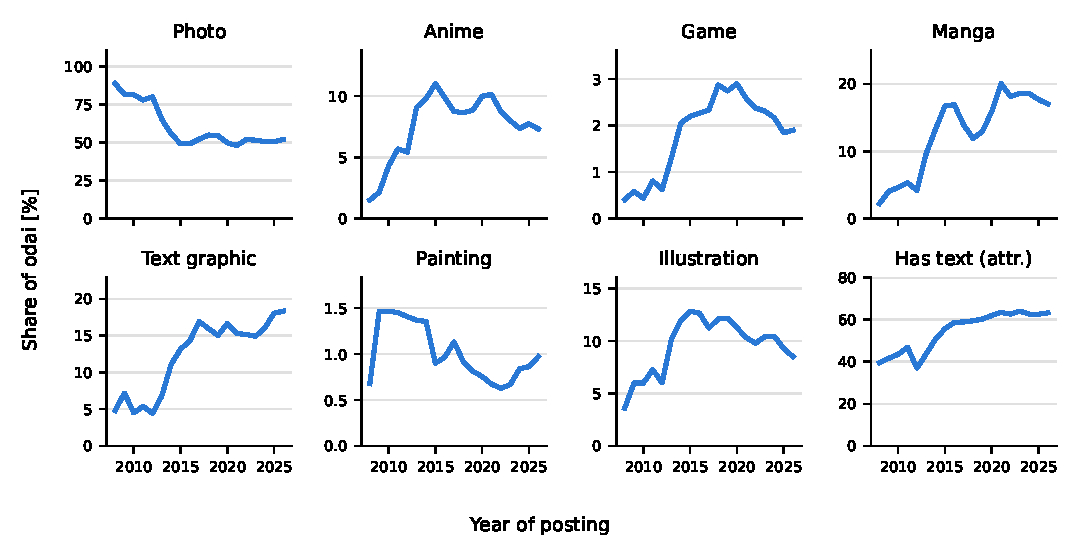
\includegraphics[width=0.85\textwidth]{figures/fig_full_year_media.pdf}
    \caption{投稿年ごとの媒体と文字ありの割合．Photo は写真，Anime はアニメ，Game はゲーム，Manga はマンガ，Text graphic はテキストグラフィック，Painting は絵画，Illustration はイラスト，Has text は属性の文字ありを表す}
    \label{fig_full_year_media}
\end{figure*}

写真の割合は2008年の約89\%から2015年の約49\%まで下がり，その後は約50\%で推移している．
代わりに，アニメ，マンガ，テキストグラフィック，イラストの割合が2013年から2015年にかけて増えた．
文字ありの割合も約40\%から約60\%に増えており，お題画像は写真に一言を付けるものから，文字や作品の画像を用いるものへと多様化したといえる．
ただし，これらの推移は生徒の予測に基づくものであり，年ごとの精度の違いは評価していない．
